\documentclass[10pt,twocolumn,letterpaper]{article}
\usepackage[review]{cvpr}
\usepackage{times,graphicx,amsmath,amssymb,booktabs,tabularx,float}
\usepackage[T1]{fontenc}
\usepackage{microtype}
\definecolor{cvprblue}{rgb}{0.15,0.43,0.64}
\usepackage[breaklinks,colorlinks,allcolors=cvprblue]{hyperref}
\def\paperID{Draft}
\def\confName{CVPR}
\def\confYear{2026}
\title{BrickAtlas: A Benchmark for Visual Evidence Following\\
Supplementary Material}
\author{Anonymous submission}
\begin{document}
\maketitle
\raggedbottom

\section{Resource and Observation Inventory}
This supplement documents the source collection, exact visual
observations, assignment audits, qualification protocol and supporting
graph controls. It accompanies the current benchmark manuscript.
The primary visual dataset remains \texttt{brickatlas-display-v3};
subsequent measurement audits do not create a new stimulus version.
The 15-model experiment design is a proposal, independent of the
sealed earlier three-model study.

The 24 human-authored LDraw sources contain 15,334 placed parts.
Source URLs, credits, licenses, original files and hashes are retained.
The 617 historical dossiers preserve questions and inspection actions.
Only 140 parents contribute primary visual pairs: 73 Color and
67 Part-type. Table~\ref{tab:sources} lists their source coverage.
Table~\ref{tab:scale} groups the historical resource by assembly scale.
The scale bands are not validated cognitive-difficulty levels.

\begin{table}[H]
\centering\small
\caption{Source scale and historical item counts. These item counts
must not be interpreted as primary paired observations.}
\label{tab:scale}
\begin{tabular}{@{}lrrr@{}}
\toprule
Source band & Sources & Parts & Items\\
\midrule
D1 & 5 & 501 & 83\\
D2 & 9 & 2,172 & 175\\
D3 & 2 & 1,440 & 59\\
D4 & 8 & 11,221 & 300\\
\bottomrule
\end{tabular}

\end{table}

\begin{table*}[t]
\centering\small
\caption{All 24 source assemblies. Color and Part-type counts are
parents, each contributing exactly one primary pair. Shared parts,
authors and derived observations do not increase source count.}
\label{tab:sources}
\begin{tabular}{@{}llrrrr@{}}
\toprule
Source & Name & Band & Parts & Color & Part-type\\
\midrule
31028 & Sea Plane & D1 & 53 & 2 & 2\\
31027 & Blue Racer & D1 & 67 & 2 & 2\\
10156 & LEGO Truck & D1 & 111 & 2 & 1\\
omr-42102 & Mini CLAAS XERION & D1 & 129 & 2 & 1\\
omr-42020 & Twin-Rotor Helicopter & D1 & 141 & 2 & 1\\
10036 & Pizza To Go & D2 & 166 & 2 & 2\\
10014 & Caboose & D2 & 170 & 2 & 2\\
omr-31031 & Rainforest Animals & D2 & 215 & 2 & 2\\
omr-31088 & Deep Sea Creatures & D2 & 230 & 2 & 1\\
omr-42004 & Mini Backhoe Loader & D2 & 246 & 2 & 2\\
omr-42061 & Telehandler & D2 & 261 & 2 & 2\\
31009 & Small Cottage & D2 & 270 & 2 & 1\\
5867 & Super Speedster & D2 & 278 & 2 & 2\\
10128 & Train Level Crossing & D2 & 336 & 2 & 2\\
10159 & City Airport & D3 & 592 & 3 & 3\\
10001 & Metroliner & D3 & 848 & 4 & 4\\
omr-10269 & Harley-Davidson Fat Boy & D4 & 1029 & 4 & 4\\
omr-10242 & MINI Cooper & D4 & 1086 & 4 & 4\\
omr-42066 & Air Race Jet & D4 & 1244 & 5 & 5\\
10213 & Shuttle Adventure & D4 & 1254 & 5 & 5\\
omr-10265 & Ford Mustang & D4 & 1357 & 5 & 5\\
10220 & Volkswagen T1 Camper Van & D4 & 1428 & 5 & 4\\
omr-21309 & NASA Apollo Saturn V & D4 & 1845 & 5 & 5\\
omr-42054 & CLAAS XERION 5000 TRAC VC & D4 & 1978 & 5 & 5\\
\bottomrule
\end{tabular}

\end{table*}

\subsection{Exact input boundary}
An observation binds the complete system and user messages, question,
options and native 1280$\times$800 image. The internal record retains
its observation ID, source identity, display mapping, condition and
gold. The model-visible input does not expose these audit fields.
All labels resolve inside the current image. The prescribed output
is exactly one JSON object containing one listed \texttt{choiceId}.

Changes to text, options, image bytes, dimensions or image policy
require renewed qualification of affected observations. Provider
envelopes additionally record requested model revision, adapter,
generation settings and full request hash. The provider's internal
image preprocessing is not directly observed. A matching local
envelope therefore establishes the delivered request, not every
internal transformation.

\subsection{Concrete visual pair}
For OMR 42004, Color asks for the current color of B0035.
The displayed answer is Blue in A and Red in B; the original source
record stores Black. The image-local contract explicitly permits
edited appearance.
Part-type retains B0035 as target. Candidate B0036 selects the
matching source type, 32250, in A. After B0036 and B0116 exchange
referents, B0116 selects that same geometry in B.
This is a change in the correct reference, not a change in the
canonical part's type.

The main figure uses these actual PNGs with identical crop rectangles
within each family. Gold annotations belong only to the publication.
The copied \texttt{figure-provenance.json} identifies original
observations, PNG hashes and crop rectangles, and
\texttt{asset-provenance.json} binds the current publication assets
to their archived source bytes. There are no fabricated model
responses in the figure.

\subsection{Appearance baseline}
The legal Color baseline accepts one wire containing only PNG and
text/options. It runs in a fresh isolated process with an empty working
directory. The evaluator joins IDs and independently reconstructed
gold afterward. No private masks, paths, source facts or counterparts
are supplied to the predictor.

RGB channels are normalized to $[0,1]$. Near-white pixels with all
channels at least .90 are removed. Pixels whose maximum channel
is at most .30 vote Black. Other pixels require saturation at least
.35 and hue within $60^\circ$ of the nearest prototype: Red at
$0^\circ$, Blue at $240^\circ$, or Yellow at $60^\circ$.
Within each category, four-connected components smaller than the
greater of 64 pixels and .0005 of image area are removed.
The winning category requires .55 of retained support; ties and
empty support abstain. Thresholds were locally committed before
the corpus run after synthetic tests.

The measured result is 141/146 correct endpoints, five abstentions
and 68/73 Both (93.15\% micro; 91.875\% equal-source).
This baseline summarizes rendered appearance across the image;
it does not locate the target label or validate multi-object
reference following. Per-observation support and failure records
are available with the audit.

\begin{figure*}[t]
\centering
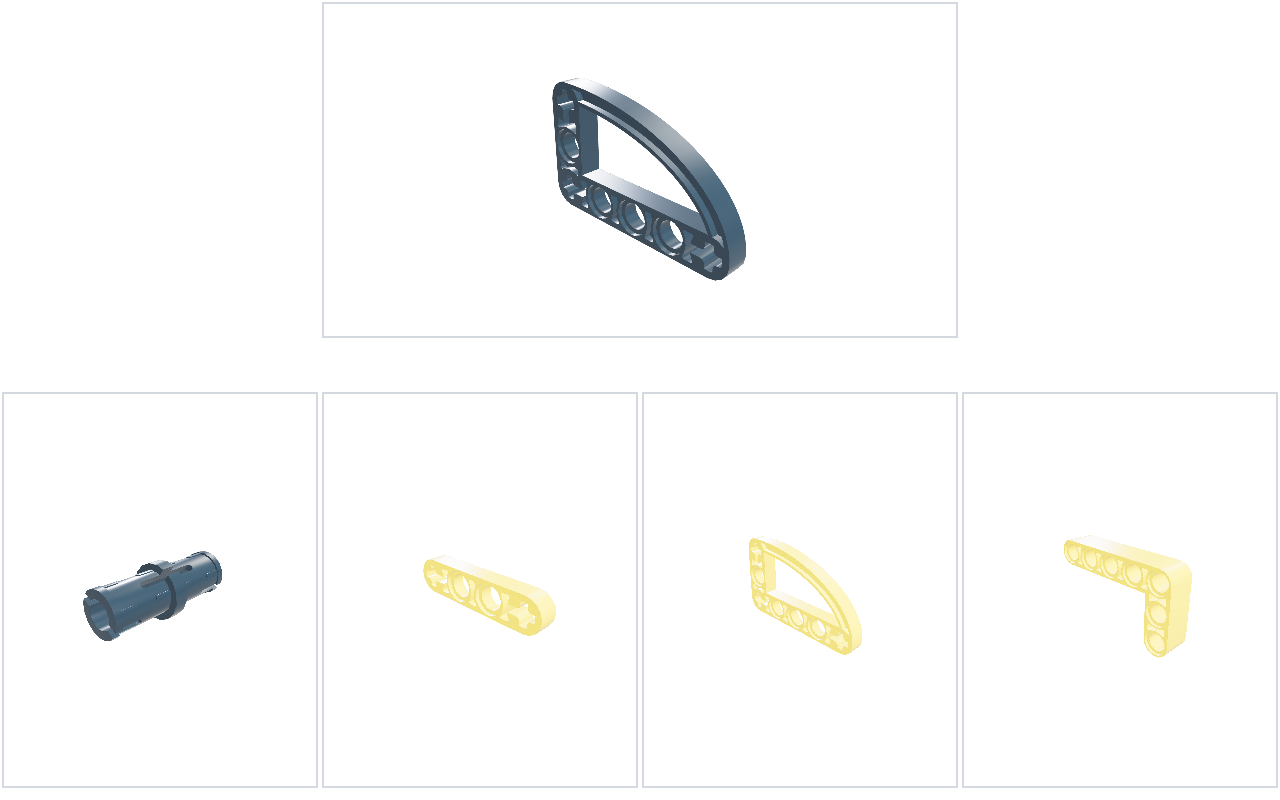
\includegraphics[width=.75\textwidth]{figures/position-control.png}
\caption{Complete auxiliary position-reference input for OMR 42004.
The target is above four candidates; the matching candidate is third
from the left. No labels appear inside the image. These isolated
parts are observations, not a proposed freestanding assembly.
The panel comparison changes layout and visual access together.}
\label{fig:panel}
\end{figure*}

\section{Part-type Assignment and Priors}
Admissible configurations enumerate all four-option permutations
and nonmatching swaps with an on-screen anchor and unique source-type
match. The 4,824 configurations are ordered by parent, option-label
tuple and swap. Constraint-equivalent choices keep the minimum integer
hash cost, leaving 2,412 variables.
One configuration is selected per parent subject to the stated
option, transition and shortcut bounds.
The recorded single-thread SciPy 1.17.1/HiGHS solution has objective
1,007,668 with zero relative gap. The frozen assignment, rather than
runtime-dependent regeneration, defines the released dataset.

\begin{table}[H]
\centering\small
\caption{A-to-B choice transitions. Rows are A gold, columns B gold.
Left: Color (73 pairs); right: Part-type (67 pairs).
Balanced semantic colors do not imply balanced option transitions.}
\begin{tabular}{@{}lrrrr@{}}
\toprule
$A\backslash B$ & A & B & C & D\\
\midrule
A & 0 & 3 & 3 & 7\\
B & 7 & 0 & 7 & 8\\
C & 4 & 8 & 0 & 7\\
D & 5 & 4 & 10 & 0\\
\bottomrule
\end{tabular}
\hspace{10pt}
\begin{tabular}{@{}lrrrr@{}}
\toprule
$A\backslash B$ & A & B & C & D\\
\midrule
A & 0 & 6 & 5 & 5\\
B & 6 & 0 & 6 & 5\\
C & 5 & 6 & 0 & 6\\
D & 6 & 5 & 6 & 0\\
\bottomrule
\end{tabular}

\end{table}

\begin{table}[H]
\centering\small
\caption{All declared Part-type oracle-A rules: B accuracy (\%).
A gold is supplied, so B accuracy equals Both. These are privileged
construction audits; their intervals are descriptive after assignment.}
\setlength{\tabcolsep}{3pt}
\begin{tabular}{@{}lrrl@{}}
\toprule
Oracle-A rule & Micro & Source & Source 95\% CI\\
\midrule
First alternative & 34.33 & 26.94 & [15.62, 38.61]\\
Last alternative & 32.84 & 32.01 & [19.93, 44.86]\\
Cyclic next & 35.82 & 38.68 & [25.00, 53.33]\\
Cyclic previous & 34.33 & 28.89 & [17.92, 40.35]\\
Cyclic two & 29.85 & 32.43 & [19.79, 46.25]\\
Smallest alternate label & 29.85 & 24.58 & [14.58, 34.38]\\
Largest alternate label & 38.81 & 39.03 & [26.04, 52.50]\\
Nearest label number & 29.85 & 30.42 & [18.75, 43.12]\\
Farthest label number & 31.34 & 29.03 & [17.08, 41.53]\\
Nearest source center & 29.85 & 36.60 & [23.61, 50.97]\\
Farthest source center & 35.82 & 28.75 & [17.92, 40.21]\\
Nearest projected anchor & 25.37 & 30.14 & [17.36, 44.38]\\
Farthest projected anchor & 32.84 & 27.08 & [16.25, 38.75]\\
\bottomrule
\end{tabular}

\end{table}

Rules use first/last alternative, cyclic option position, alternate
label-number extrema, distance from target label number, or
nearest/farthest source center or projected anchor. Ties use
ascending original numeric labels. Spatial rules use evaluator-side
geometry. None reads B pixels, and no rule supplies a universal model
ceiling. Independent reconstruction checks golds and features against
source records and rendering metadata.

\section{Human Qualification}
\subsection{Assignment and raw records}
Six packages contain 115, 116, 114, 115, 115 and 119 judgments.
Their union covers all 347 observations exactly twice. Reviewers
must be distinct people, and each sees at most one observation of
any parent, including the panel control. Three-observation parents
therefore use all six reviewers. Queues are shuffled and use opaque
unit IDs without condition or arm labels.

A raw record contains the reviewer pseudonym, timestamp, observation
hash, visual choice, categorical decision, four structured checks,
reason, native-size inspection attestation and independence attestation.
The four checks concern a unique target, unique visual answer,
sufficient visibility and absence of reference contradictions.
Decidable judgments require a listed choice and all checks passing.
Other decisions require an exclusion reason. The interface hides
gold, source data, counterpart, model output and other reviewers'
judgments. The coordinator retains unmodified exports.

\subsection{Adjudication and denominators}
Agreement on decision, choice and checks permits finalization.
Any disagreement on these fields requires an additional independent
adjudicator. Up to three adjudicator slots preserve parent-disjoint
exposure and exclude initial reviewers. The adjudicator sees the
single observation and its two judgments, but not gold, another
observation of that parent or model outputs.
Original records remain intact. A final decidable choice that
conflicts with generated gold blocks finalization and requires
stimulus revision and renewed review.

The full primary universe is always 280 endpoints and 140 pairs.
There are 560 initial primary judgments and 134 auxiliary judgments.
Actual collected judgments are currently zero. The runner's existing
full-study gate requires final decisions for every planned endpoint.
Nondecidable cases remain in full-set scoring; the additional
qualified subset requires two decidable endpoints per pair.
A new MVP needs a separate frozen subset with valid review lineage,
not an override of the full-study gate.

Raw categorical agreement and choice/check agreement use their
actual eligible denominators. Pooled two-slot Cohen's kappa is
$(p_o-p_e)/(1-p_e)$ from empirical decision marginals.
Because assigned people vary across observations, it is not the
reliability of one fixed reviewer pair. Missing judgments or
degenerate expected agreement produce undefined kappa.
Adjudicated agreement cannot replace the raw measure.

\section{Scoring and Dependence}
The four B outcomes partition every changed-answer pair: correct
new gold, valid old gold, another valid answer, and invalid output.
Missing calls are invalid and remain in the fixed denominator.
AAcc and Both retain information about A correctness.
Conditional adaptation reports the number of A-correct pairs and
the sources with at least one eligible pair.

Equal-source estimates average within-source means. The bootstrap
resamples whole sources 10,000 times using seed 20260920.
Model contrasts use the same pairs. Qualified-minus-full contrasts
reuse source weights and recompute means on eligible sources.
An empty subset or a draw containing no eligible source is
recorded as undefined.
No whole-source interval estimates provider randomness across repeats.
Boundary outcomes can yield degenerate intervals.

The 24 sources form 18 primary-author and 17 contributor-connected
groups. Contributor groups include credited OMR editors.
Sensitivity analysis averages within-source outcomes by author,
resamples whole author groups and omits each author in turn.
Direction changes under omission limit stability claims.
The public inventory additionally contains all 276 source-pair
part-count and part-set Jaccards; these are inventory similarities,
not spatially aligned geometry overlaps.

\begin{table}[H]
\centering\small
\caption{Repeated primary authors. Other primary-author groups
contain one source each.}
\begin{tabular}{@{}ll@{}}
\toprule
Repeated primary author & Source IDs\\
\midrule
Merlijn Wissink & 31027, 31028\\
Philippe Hurbain & 42054, 42061, 42066\\
Robert Paciorek & 10036, 10128, 10156\\
Zoltan Keri & 10001, 10159\\
\bottomrule
\end{tabular}

\end{table}

\begin{table}[H]
\centering\small
\caption{Largest part-inventory overlaps. Count Jaccard uses summed
per-type minima divided by summed maxima; set Jaccard ignores counts.}
\begin{tabular}{@{}llrr@{}}
\toprule
Source A & Source B & Count J. & Set J.\\
\midrule
42054 & 42066 & 0.450 & 0.511\\
42004 & 42061 & 0.370 & 0.354\\
42004 & 42020 & 0.325 & 0.431\\
10220 & 10242 & 0.322 & 0.257\\
10265 & 10269 & 0.280 & 0.320\\
\bottomrule
\end{tabular}

\end{table}

\section{Graph Construction and Completed Algorithm Audits}
Graph questions provide explicit undirected edge lists and a node
to delete. Repeated edges are deduplicated; surviving isolates count
as components. Independent BFS and union-find agree on all golds.
These checks validate the supplied graph operation, not completeness
of physical connector detection.

The hypothetical collection has 219 distinct observations: an anchor,
a changed partner and an isomorphic invariant partner for each of
73 parents. Strong change contains 12 pairs from eight sources;
degree-visible change contains 61 from 23 sources. Each has a
corresponding invariance partition. Pair endpoints therefore have
292 appearances across all partitions, but only 219 unique inputs.

\begin{table*}[t]
\centering\small
\caption{Completed deterministic algorithm audit. These values are
computed algorithm outputs, not planned or measured language-model
results. Natural and hypothetical lookups use separate source-held-out
fits. Invariance shares anchors with change.}
\begin{tabular}{@{}lrrrr@{}}
\toprule
Algorithm & \shortstack{Natural\\correct / 73} & \shortstack{Strong change\\Both / 12} & \shortstack{Degree-visible\\Both / 61} & \shortstack{Strong invariance\\Both / 12}\\
\midrule
Node-count lookup & 63 & 0 & 0 & 6\\
Edge-count lookup & 44 & 0 & 0 & 7\\
Degree-histogram lookup & 69 & 0 & 61 & 6\\
Anonymous 1-WL lookup & 69 & 0 & 61 & 6\\
Isolates + one & 72 & 0 & 61 & 6\\
BFS & 73 & 12 & 61 & 12\\
Union-find & 73 & 12 & 61 & 12\\
\bottomrule
\end{tabular}

\end{table*}

\begin{table}[H]
\centering\small
\caption{All strong changed-answer pairs, with matching surviving
nodes, edge count, target degree, degree multiset and isolate count.
BFS and union-find have Both=1 on each.}
\begin{tabular}{@{}lrrr@{}}
\toprule
Parent task & $y_A$ & $y_B$ & Isolates+1 Both\\
\midrule
ld2-10001-graph-removal-4 & 2 & 3 & 0\\
ld2-10014-graph-removal-1 & 2 & 3 & 0\\
ld2-10014-graph-removal-2 & 1 & 2 & 0\\
ld2-10213-graph-removal-1 & 4 & 3 & 0\\
ld2-31009-graph-removal-2 & 4 & 3 & 0\\
ld2-5867-graph-removal-1 & 1 & 2 & 0\\
ld2-omr-10269-graph-removal-1 & 2 & 1 & 0\\
ld2-omr-10269-graph-removal-2 & 2 & 1 & 0\\
ld2-omr-10269-graph-removal-4 & 2 & 1 & 0\\
ld2-omr-21309-graph-removal-2 & 2 & 3 & 0\\
ld2-omr-21309-graph-removal-4 & 2 & 1 & 0\\
ld2-omr-42054-graph-removal-4 & 3 & 4 & 0\\
\bottomrule
\end{tabular}

\end{table}

The strong construction compares a six-cycle and two triangles plus
identical isolated nodes. The weaker construction compares a path
and a triangle plus isolates. Only the former matches the complete
degree multiset. Uniform-feature anonymous 1-WL signatures collide
on every strong pair, so a deterministic signature-only predictor
cannot answer both different golds correctly.
Unique node identifiers, positional features, spectral features and
higher-order models lie outside this restriction.

Feature lookups train only on other sources, choose the most frequent
answer, break ties toward the smaller integer and abstain on unseen
features. Abstention is incorrect. Hypothetical fitting includes the
changed endpoints once and excludes invariant duplicates.
The isolates-plus-one heuristic predicts the isolate count plus one
when any nonisolated node remains; it never traverses components.

\begin{table}[H]
\centering\small
\caption{Completed invariance algorithm audit. Repeating a wrong
answer is consistent but fails Both.}
\begin{tabular}{@{}lrr@{}}
\toprule
Algorithm & Strong / 12 & Degree-visible / 61\\
\midrule
Node-count lookup & 6 & 31\\
Edge-count lookup & 7 & 32\\
Degree-histogram lookup & 6 & 61\\
Anonymous 1-WL lookup & 6 & 61\\
Isolates + one & 6 & 61\\
BFS & 12 & 61\\
Union-find & 12 & 61\\
\bottomrule
\end{tabular}

\end{table}

Strong change has six increases and six decreases in gold component
count; arm-wise answer histograms need not match. Both is invariant
to swapping A and B. Wilson intervals for 0/12 and 12/12 are
approximately $[0,.2425]$ and $[.7575,1]$ under a pair-independence
approximation that source reuse violates. The single template and
eight-source coverage limit generalization.

\begin{figure*}[t]
\centering
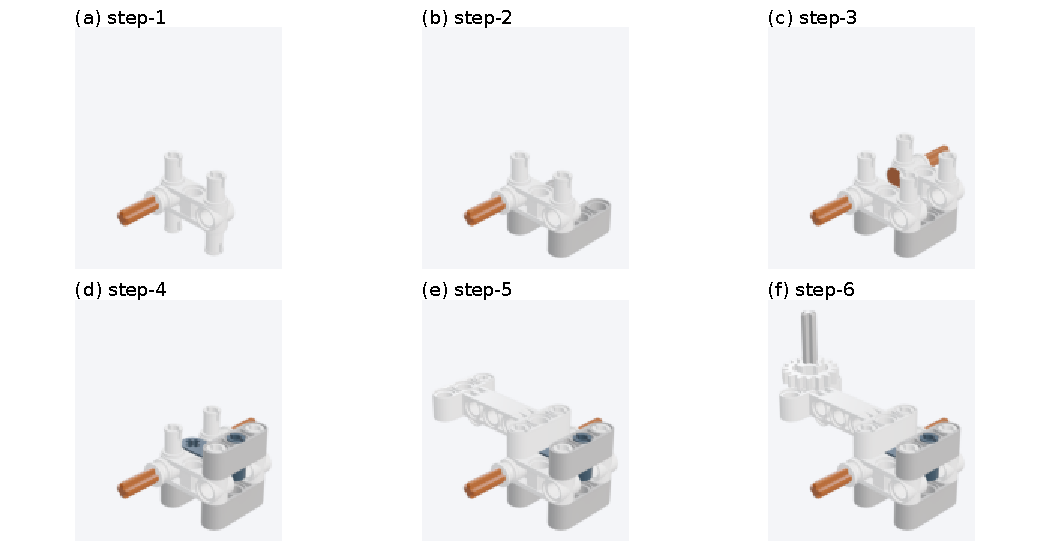
\includegraphics[width=.78\textwidth]{figures/given-order-replay.pdf}
\caption{Historical given-order 3D visibility replay for set 42102.
Parts appear at their saved source transforms. The supplied sequence
is an inspection control, not a discovered model plan; it does not
certify an insertion path or gravity stability.}
\end{figure*}

\section{Collection and Publication Contract}
The main paper lists 15 proposed models and 306 empty result cells
across primary visual, diagnostic, control, graph and mode tables.
The model inventory comes from the existing budget snapshot.
All result values in \texttt{experiments.json} are null and render
as empty cells. Null represents uncollected results, not measured
zero or an unspecified model name.

Before collection, the new study must freeze selected IDs, exact
models and revisions, provider/precision, adapter code, image policy,
output and effort settings, repeat count, timeouts, inclusion and
failure policies, and qualification lineage. The MVP proposal keeps
complete visual pairs and all three observations of each selected
graph parent. It requires new adapters and a subset qualification
gate; those implementation steps remain open.

The earlier sealed evaluator fixes three models and nine runs.
It cannot silently accept the new roster. Its receipt reconstruction,
failure denominators and source estimators provide implementation
references, while the new study requires its own versioned manifest.
No synthetic fixture, dry run, historical response or missing
receipt can substitute for a genuine observation in empirical tables.
Real response cases must link to exact requests and retained outputs;
an absent failure category remains absent.

Current manuscript files are under \texttt{paper/}; code and dataset
indexes are under \texttt{benchmark/}. Intermediate reviews, guidance
and manuscripts are physically archived under \texttt{tem/}, with
compatibility links for historical paths. Git includes data, image
assets, reviewer packages, code and PDFs. Redundant local recovery
tarballs and runtimes are excluded; full historical recovery checks
require those separate bundles. Hashes establish local consistency,
while genuine human independence and provider origin additionally
require collection oversight.
\end{document}
